\documentclass[11pt]{beamer}
\setbeamertemplate{navigation symbols}{}%remove navigation symbols
\usepackage{booktabs}
\usepackage{hyperref}
\usepackage{subfig}
\usepackage{tcolorbox}

\usefonttheme{professionalfonts}
%\usefonttheme{serif}

%\usepackage{fontspec}
%\usepackage{kantlipsum}
\setbeamerfont{note page}{family*=pplx,size=\footnotesize}
\useoutertheme{infolines}

\usepackage[framemethod=tikz]{mdframed}
\usetikzlibrary{shadows}
\usepackage{pdfpages}
\newmdenv[shadow=true,shadowcolor=black,font=\sffamily,rightmargin=8pt]{shadedbox}
\usepackage{pifont,xcolor}% http://ctan.org/pkg/{pifont,xcolor}
\definecolor{myblue}{RGB}{49,54,149}
\definecolor{myred}{RGB}{165,0,38}
\usepackage{graphicx}
\usepackage{caption}
\newcommand{\lenitem}[2][.55\linewidth]{\parbox[t]{#1}{#2\strut \strut}}

\usetheme{Frankfurt}

   \usefonttheme{professionalfonts} 
\newenvironment{variableblock}[3]{%
  \setbeamercolor{block body}{#2}
  \setbeamercolor{block title}{#3}
  \begin{block}{#1}}{\end{block}}
\usecolortheme{dove}
\usepackage{fancybox}
\setbeamercolor{block title}{bg=white,fg=black}
\newenvironment{fminipage}%
{\begin{Sbox}\begin{minipage}}%
{\end{minipage}\end{Sbox}\fbox{\TheSbox}}

\newcommand{\itemcolor}[1]{% Update list item colour
  \renewcommand{\makelabel}[1]{\color{#1}\hfil ##1}}

\newcounter{tmpc}
%\usefonttheme{structuresmallcapsserif}
\setbeamercolor{section in head/foot}{fg=black, bg=white}
\setbeamercolor{enumerate item}{ fg=red}
\setbeamertemplate{frametitle}
{
    \nointerlineskip
    \begin{beamercolorbox}[sep=0.3cm,ht=1.8em,wd=\paperwidth]{frametitle}
        \vbox{}\vskip-3ex%
        \strut\insertframetitle\strut
        \vskip-1.2ex%
    \end{beamercolorbox}
}
\addtobeamertemplate{frametitle}{\vskip0.5ex}{}
\makeatletter
\setbeamertemplate{footline}
{
  \leavevmode%
  \hbox{%
  \begin{beamercolorbox}[wd=.875 \paperwidth,ht=2.25ex,dp=1ex,left]{section in head/foot}%
    \usebeamerfont{author in head/foot}\quad \quad \insertshorttitle
 \end{beamercolorbox}%
 \begin{beamercolorbox}[wd=.125\paperwidth,ht=2.25ex,dp=1ex,right]{section in head/foot}%
    \usebeamerfont{date in head/foot} \quad \quad
    \insertframenumber{} / \inserttotalframenumber\hspace*{2ex} 
  \end{beamercolorbox}}%
  \vskip0pt%
}
\let\@@magyar@captionfix\relax
\makeatother

\def\mf{
\begin{itemize}
\item Item
\end{itemize}
}
%\setbeamercolor{itemize item}{fg=yellow,bg=white}
%\setbeamertemplate{itemize items}[circle]
\setbeamercolor{enumerate item}{ fg=red}
\setbeamercolor{item projected}{bg=myblue}

\usepackage{listings}

\lstdefinestyle{BashInputStyle}{
  language=bash,
  basicstyle=\small\sffamily,
  numbers=left,
  numberstyle=\tiny,
  numbersep=5pt,
  framexleftmargin=3mm,
  frame=shadowbox, rulesepcolor=\color{gray},
  numberstyle=\normalfont\tiny\color{myred},
%  fillcolor=\color{gray},
  rulecolor=\color{black},
  columns=fullflexible,
  backgroundcolor=\color{white},
  linewidth=0.9\linewidth,
  xleftmargin=0.1\linewidth
}


\begin{document}

\section{Title/Intro}
\subsection{}
\small
\title{The Architecture of Genome Wide Study\vspace{-.2in}} 
\author{Melinda C. Mills and \textbf{Charles Rahal}\\ Department of Sociology and Nuffield College \\ University of Oxford \\ \vspace{0.1in} Departmental Seminar, 11th June, 2018}
 \date{}
\frame{\titlepage 
\begin{center}
 \vspace{-0.5in}
 \includegraphics[width=0.5\textwidth]{helix_wordcloud_1250_5000_black.pdf}\\ \vspace{0.2in}
%\color{myblue}Postdoctoral Seminar -- Nuffield College \color{black}\\ \vspace{0.1in}
Replication/Supplementary Material: \color{myblue}\url{https://github.com/crahal}\color{black}\\ 
%Comments/Questions/Suggestions: \color{myred}\url{charles.rahal@sociology.ox.ac.uk}\\
 \end{center}
}

\subsection{}
\frame{
\frametitle{General Introduction}
Most speakers in this series present multiple papers or summarize their work/field. \\ \vspace{0.1in} 
My interests are extremely varied in general. Some specific examples:\vspace{0.05in} 
\begin{itemize}
\item Civic Technology (public procurement and corporate lobbying).
\item Social Mobility and Mortality (applied projects focusing on `elites').
\item Residential Market Policies (discrimination and affordability).
\item Econometric Methods (mostly spatial and time series).
\item ... and of course, Socio-genomics and the Sociology of Genomics.  \\ \vspace{0.1in}
\end{itemize}
Unifying themes: unstructured data, `big data', methodological advancements.\\ \vspace{0.1in}
However, today we'll just focus on one paper: `The Architecture of GWAS'. \\ \vspace{0.1in}
Come to Belfast next week to see a talk on the \color{myred}\url{centgovspend}\color{black}{ }project!
}


\subsection{}
\frame{
\frametitle{One thing I'm especially interested in...}
\footnotesize
\begin{itemize}
\item We're (slowly) entering the replication era in social science.
\footnotesize
\item Open-source: sometimes before it's published! Everything you'll see today:
\setbeamertemplate{enumerate items}[default]
\begin{enumerate}
\footnotesize
\item Uses open-source general purpose programming (i.e. Python 3.6).
\item Is presented using an open source typesetting engine (i.e. XeLaTeX).
\item Makes use of free, easily accessible data sources (i.e. PubMed).
\item Is hosted online and can be replicated by anyone (i.e.  \color{myred}\url{GitHub}).
\end{enumerate}
\end{itemize}\vspace{-.15in}
\normalsize
\begin{figure}
\centering
%\begin{minipage}{.5\textwidth}
%  \centering
\hspace{-.3in}  \includegraphics[width=.75\linewidth]{github1b.png}
%  \label{fig:test1}
%\end{minipage}\hspace{-.15in}
%\begin{minipage}{.5\textwidth}
%  \centering
%  \includegraphics[width=.92565\linewidth]{github2.png}
%  \label{fig:test2}
%\end{minipage}
\end{figure}
}

\subsection{}
\frame{
\frametitle{Introduction to `The Architecture of GWAS'}
\begin{itemize}
\item Joint work with Professor Melinda C. Mills. \\ \vspace{0.05in}
\item Started out as a `Genomics is WEIRD' style review, but contiunously evolved. \\ \vspace{0.05in}
\item Initiated by a `Comment' in Nature regarding GWAS participant ancestry. \\ \vspace{0.05in}
\item We systematically expand this idea in multiple directions... \\ 
\end{itemize}
\begin{figure}
\centering
\includegraphics[width=.975\linewidth]{genomicsfailingdiversity.png}
\end{figure}
}

 \subsection{}
\frame{
\frametitle{Introduction to `The Architecture of GWAS' (Cont.)}
\begin{itemize}
%\item The paper itself is now an `invited review' at Communications Biology. \\ \vspace{0.1in}
\item It represents a toolkit for analysing the (social-)architecture of GWAS. \\ \vspace{0.1in}
\item It is a data-driven response to `folk theorems' and qualitative commentaries.\\ \vspace{0.1in}
\item Key idea: link multiple data sources to understand what drives discovery.\\ \vspace{0.1in}
\item We can roughly group the conclusions we draw herein into three categories:\\
\begin{center}
 i.) Participants, ii.) Researchers and iii.) Funders.\\ \vspace{0.1in}
\end{center}

\item Mostly generalizable to all life-science and biomedical topics. \vspace{-.1in}
\end{itemize}
\begin{figure}
\centering
\begin{minipage}{.33\textwidth}
  \centering
  \includegraphics[width=.9\linewidth]{gwascatlogo.jpg}
  \label{fig:test1}
\end{minipage}%
\begin{minipage}{.33\textwidth}
  \centering
  \includegraphics[width=.9\linewidth]{pubmedlogo.png}
  \label{fig:test2}
\end{minipage}
\begin{minipage}{.33\textwidth}
  \centering
  \includegraphics[width=.9\linewidth]{EuropePMC1.png}
  \label{fig:test2}
\end{minipage}
\end{figure}
}

\subsection{}
\frame{
\frametitle{What is a \textbf{G}enome \textbf{W}ide \textbf{A}ssociation \textbf{S}tudy?}

\begin{itemize}
\item Observational studies of genome-wide sets of genetic variants.\\ \vspace{0.05in}
\item Scans associations between \textbf{S}ingle-\textbf{N}ucleotide \textbf{P}olymorphisms and traits.\\ \vspace{0.05in}
\item Traits can be related to disease (i.e. neoplasty), body measurements (ie anthropometry) or behaviour (i.e. \textbf{H}uman \textbf{R}eproductive \textbf{B}ehaviour).\\ \vspace{0.05in}
\item Individuals submit DNA to cohorts, which are combined into a \textbf{GWAMA}.\\ \vspace{0.05in}
\item A typical GWAMA will have both a \textit{discovery} and \textit{replication} sample.\\ \vspace{0.05in}
\item Specific examples include:
\begin{itemize}
\item \textbf{EA3}: N=$\sim$1.1m, R$^2$=0.11 to 0.13\% for educational attainment.
\item \textbf{HRB1}: 0.9\% for AFB and 0.2\% for NEB. HRB2 has N=$\sim$800k+.\\ \vspace{0.05in}
\end{itemize}

\item Requires substantial human and computational capital (and funding).
\end{itemize}
}
\subsection{}
\frame{
\begin{figure}
\centering
\begin{minipage}{.5\textwidth}
  \centering
  \includegraphics[width=\linewidth]{DM_header.png}
  \label{fig:test1}
\end{minipage}\hspace{.2in}
\begin{minipage}{.4\textwidth}
  \centering
  \includegraphics[width=.95\linewidth]{circular_manhatten.png}
  \label{fig:test2}
\end{minipage} \\ \vspace{0.1in}
\begin{minipage}{.9\textwidth}
  \centering
  \includegraphics[width=.85\linewidth]{manhat.png}
  \label{fig:test2}
\end{minipage}
\end{figure}

}

\subsection{}
\frame{
\frametitle{Data}
\footnotesize
\begin{itemize}
\item Starting point -- NHGRI-EBI Catalog: curated database of SNP-trait associations. 
\begin{figure}
\centering
\includegraphics[width=.8\linewidth]{GWAS_Catalog_diagram1.pdf}
\end{figure}
\item `This is literally the most utilized figure in all of genetics' (Tropf, 2018).\\ \vspace{0.05in}
\item Every two weeks, new studies are updated, periodically adding new fields.
\end{itemize}
}

\subsection{}
\frame{
\frametitle{Methods}
\begin{itemize}
\item We link the PUBMEDID field to various \textbf{A}pplication \textbf{P}rogram \textbf{I}nterfaces. \\ \vspace{0.1in}
\item All analysis is done in Python 3: specifically an \href{https://github.com/crahal/architectureofGWAS/blob/master/Code/An\%20IPython\%20Notebook\%20For\%20'The\%20Architecture\%20of\%20GWAS'.ipynb}{ \color{myblue}IPython Notebook}. \\ \vspace{0.1in}
\item Notable libraries used include matplotlib, pandas, Network-X and BioPython. \\ \vspace{0.1in}
\item We provide support functions to:
\begin{enumerate}
\setbeamercolor{enumerate subitem}{fg=red!80!black}
\setbeamertemplate{enumerate items}[default]
\item Scrape and clean the four different Catalog datasets.
\item Call and parse various APIs.
\item Perform regular expression execises to link the Catalog to API data.\\ \vspace{0.1in}
\end{enumerate}
\item A traditional data science pipeline: most of the game is wrangling.\\ \vspace{0.1in}
\item We'll focus on the outputs rather than methods: see  \color{myred}GitHub\color{black}{ }if interested!
\end{itemize}
}


\section{An Overview of GWAS}
\subsection{}
\frame{
\frametitle{Some Basic Facts About GWAS (continually evolving)}
\begin{itemize}
\item There are currently about 3,314 GWAS papers published (first 2005-03-10).\\ \vspace{0.05in}
\item However: only 10 papers were published in 2005 and 2006 combined.\\ \vspace{0.05in}
\item Represents around 4,943 Accessions across 2,909 unique Diseases/Traits.\\ \vspace{0.05in}
\item The total number of Associations found is currently: 67,230.\\ \vspace{0.05in}
\item The average number of Associations found per paper is 13.6.\\ \vspace{0.05in}
\item Mean P-Value for the strongest SNP risk allele is 1.5748e-06.\\ \vspace{0.05in}
\item The number of associations reaching the 5e-8 threshold is 33,026 (49.1\%).\\ \vspace{0.05in}
\item The journal to feature the most GWAS since 2005-03-10 is Nature Genetics.\\ \vspace{0.05in}
\item Total number of journals publishing GWAS is 436.\\ \vspace{0.05in}
\item The study with the largest number of authors has 559 authors.\\ \vspace{0.05in}
\end{itemize}
}

\subsection{}
\frame{
%\frametitle{Growth of GWAS}
\begin{center}
\begin{figure}
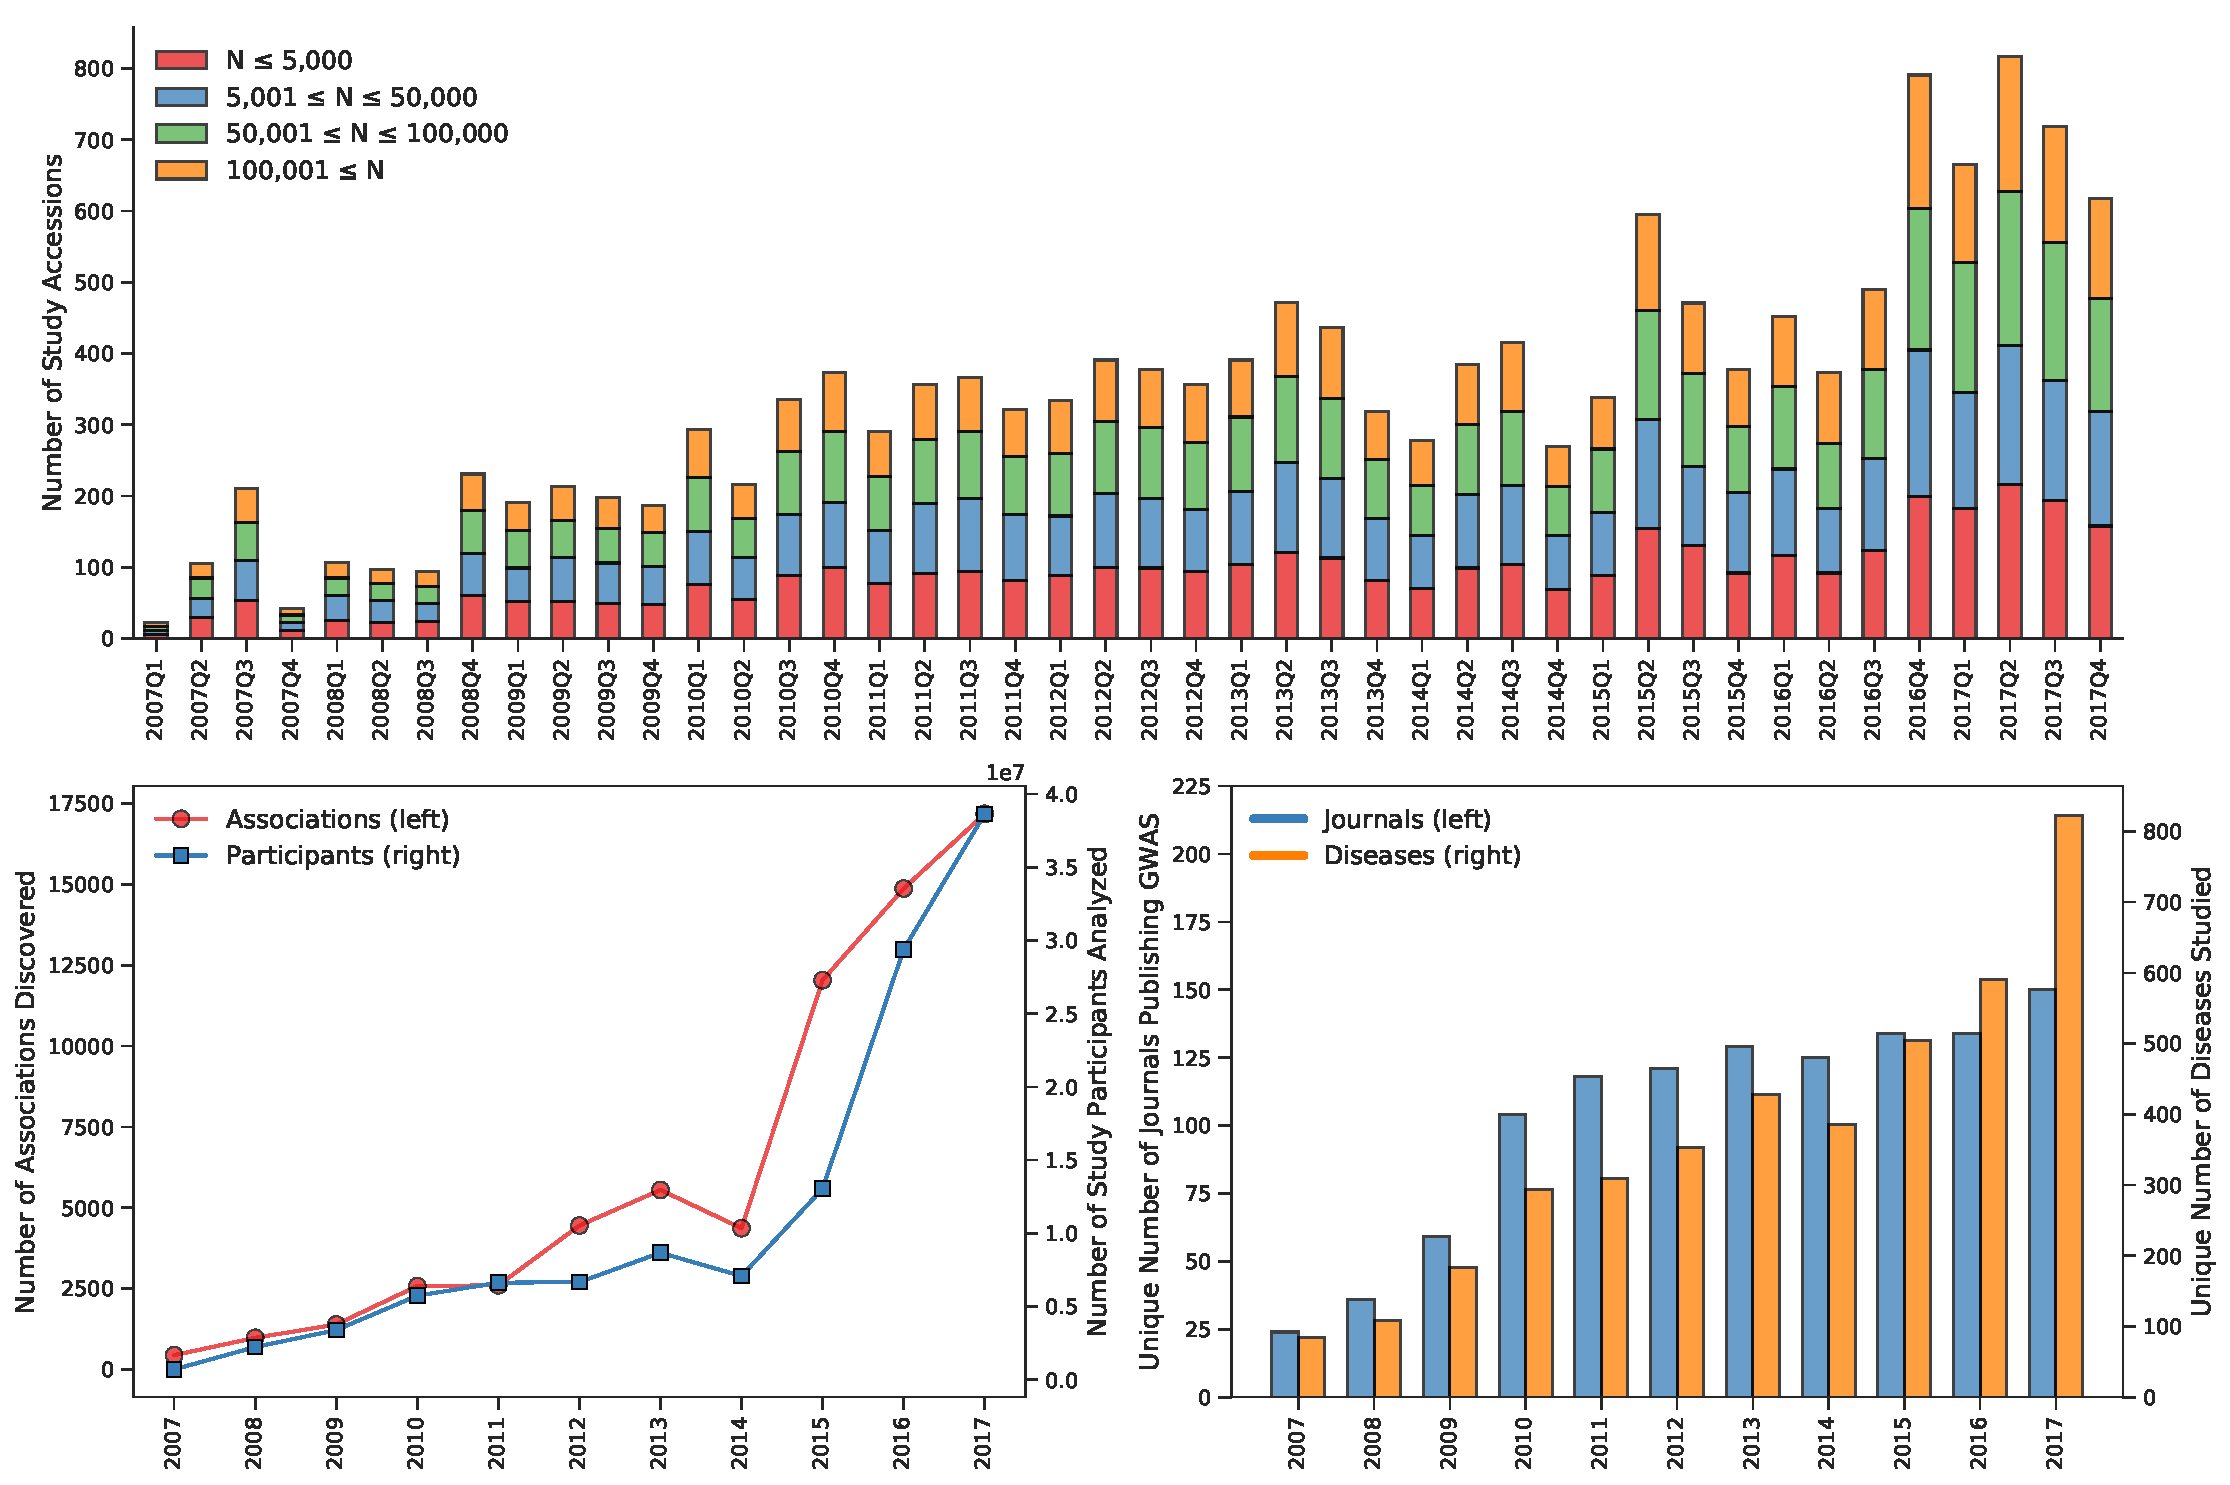
\includegraphics[width=\textwidth, angle=0]{GWAS_Popularity.pdf}
\end{figure}
\end{center}
}

\section{Participants}
\subsection{}
\frame{
%\frametitle{Participant Ancestry}
\begin{center}
\begin{figure}
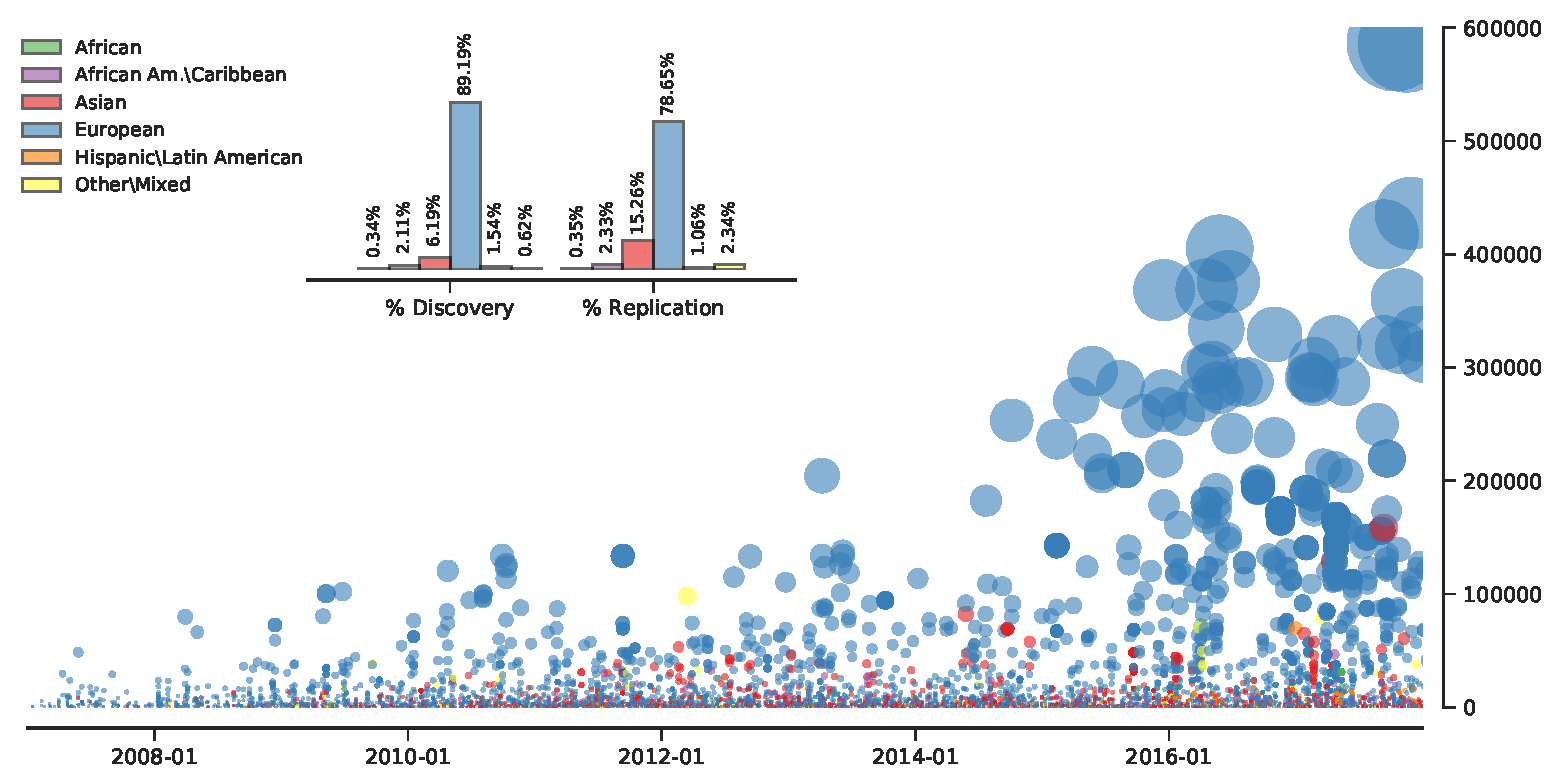
\includegraphics[width=0.975\textwidth, angle=0]{Ancestral_Plots.pdf}
\end{figure}
\end{center}
\begin{itemize}
\footnotesize
\item Public health debate about `personalized medicine': personalised for who?\\ \vspace{0.025in}
\item Larger genetic variation in non-Europeans aids discovery. Simple arithmetics shows three (four) times more discoveries per person for African (Hispanics) ancestry.
\end{itemize}
}

\subsection{}
\frame{
\frametitle{Participant Ancestry Over Time}
\begin{table}[]
\centering
\scalebox{0.85}{
\begin{tabular}{rcccccc} \toprule
     & Eur & Asian & African & H/L Am. & Other/Mixed &  AA/AC \\ \midrule
2007 & 95.47 & 2.14  & 0.01 & 0.72 & 1.18 & 0.49\\
2008 & 95.10 & 3.06  & 0.00 & 0.00 & 1.27 & 0.57\\
2009 & 88.17 & 7.10  & 0.26 & 0.22 & 3.36 & 0.88\\
2010 & 86.54 & 10.13 & 0.27 & 0.06 & 2.49 & 0.50\\
2011 & 78.19 & 15.88 & 0.15 & 0.40 & 1.72 & 3.66\\
2012 & 71.15 & 20.04 & 0.32 & 0.91 & 2.96 & 4.62\\
2013 & 81.55 & 12.10 & 0.41 & 0.82 & 0.64 & 4.48\\
2014 & 76.42 & 18.74 & 0.24 & 1.17 & 0.99 & 2.43\\
2015 & 84.47 & 11.89 & 0.37 & 0.96 & 0.66 & 1.66\\
2016 & 90.97 & 4.54  & 0.20 & 1.54 & 1.30 & 1.45\\
2017 & 88.14 & 6.29  & 0.56 & 2.30 & 0.52 & 2.19\\ \bottomrule
\end{tabular}}\\
\tiny{Abreviations: AA/AC: African American or Afro-Caribean, H/L Am: Hispanic or Latin American, Eur: European.}
\end{table}
\begin{itemize}
\item Despite a reduced focus on Europeans c.2011-2014, the upward trend is due to the rise of large national biobanks (U.K. Biobank), biopharmaceutical companies (DeCODE) and personal genetics (23andMe).
\end{itemize}
}


\subsection{}
\frame{
\frametitle{Polyvocality and Scientific Authority}

\begin{itemize}
\item Former analysis is based on a mapping between 182 combinations of `broader ancestries'  identified in the Catalog and our six pre-defined categories.\\ \vspace{0.05in}
\item The Catalog also provides a `free text' field describing the ancestry. \\ \vspace{0.05in}
\item Decompose this to examine `polyvocality' (Panofsky and Bliss, 2017, ASR). \\ \vspace{0.05in}
\item Lets take an example: 
\begin{enumerate}
\setbeamercolor{enumerate subitem}{fg=red!80!black}
\setbeamertemplate{enumerate items}[default]
\item Free text: “19,546 British ancestry individuals from 6,863 families”. \\
\item REs can separate: “19,546” and “British” into two fields for further analysis. \\ \vspace{0.05in}
\end{enumerate}
\item Isolates 207 and 147 unique terms for discovery and replication. Examples include `Caribbean Hispanic', various Chinese ancestries (Hui, Han, etc.). \\ \vspace{0.05in}
\item These classify participants in terms of race, ethnicity or ancestry. \\ \vspace{0.05in}
\item Whether these terms are used in ‘logically ambiguous ways’ to propogate authority is for somebody else to decide: but we provide a better toolkit...
\end{itemize}
}


\subsection{}
\frame{
\frametitle{Country of Recruitment}
\begin{center}
\begin{figure}
\includegraphics[width=0.95\textwidth, angle=0]{Country_Rec_N.pdf}
\end{figure}
\end{center}
}


\subsection{}
\frame{
\frametitle{Continent of Recruitment}
\begin{table}[]
\centering
\scalebox{0.85}{
\begin{tabular}{rcccc} \toprule
Continent & N & \# Studies & N (\%) & \# Studies (\%)\\ \midrule
Africa & 39,742 & 43 & 0.11 & 0.80\\
Asia & 5,180,891 & 1,298 & 14.22 & 24.11\\
Europe & 21,529,123 & 1,528 & 59.11 & 28.38 \\
North America & 9,345,005 & 2,380 & 25.66 & 44.21\\
Oceania & 302,888 & 107 & 0.83 & 1.99 \\
Seven seas & 1,389 & 1 & 0.00 & 0.02 \\
South America & 22,256 & 27 & 0.06 & 0.50\\ \bottomrule
\end{tabular}}
\end{table}
\begin{itemize}
\vspace{0.1in}
\item 0.11\% of participants recruited from Africa, 0.06\% from South America. \\ \vspace{0.05in}
\item 84.77\% of participants come from either North America or Europe.\\ \vspace{0.05in}
\item Approximately 76.2\% of the global population reside in Asia or Africa!\\ \vspace{0.05in}
\item Whether the launch of the African Genome Variation Project or China Kadoori Biobank changes this remains to be seen...
\end{itemize}
}


\subsection{}
\frame{
\frametitle{Cohort Resampling}
\begin{table}[]
\centering
\scalebox{0.85}{
\begin{tabular}{rccccc} \toprule
Cohort & Count & N       & Recruitment     & Age Range \\ \midrule
Rotterdam Study & 373   & 14,926  & Netherlands     & 55-106\\
ARIC & 187   & 15,792  & US & 45-64 \\
Framingham & 183   & 15,447  & US & 5-85*\\
CHS & 163 & 5,888   & US & 65+  \\
1958BC & 144 & 17,634 & UK & 0+ \\
SHIP & 120 & 4,308 & Germany & 20-79 \\
TWINSUK & 120   & 12,000  & UK, Ireland & 18-103 \\
Nurses Health Study & 112   & 121,700 & US & 30-55 \\
AGES & 110   & 30,795  & Iceland & 33-84 \\
EPIC & 108   & 521,330 & 10 EU countries & 21-83**\\ \bottomrule
\end{tabular}}\\
\footnotesize{*denotes originally 30-62 years, ** denotes variation by country.}
\end{table}
\normalsize
\begin{itemize}
\item Most frequently utilized cohorts: largest 1,000 GWAS (01/09/2017). \\
\item Required an \textbf{extensive} manual data collection exercise.\\ 
\item Analyzes demographics of cohorts which are repeatedly analyzed. \\
\item Many thanks to Pilar, Domant\`{e} and Xuejie for all their help!
\end{itemize}
}



\section{Funders}
\subsection{}
\frame{
\frametitle{Which Countries Fund GWAS?}
\begin{table}[]
\centering
\scalebox{0.85}{
\begin{tabular}{rcc} \toprule
 & \# Acknowledgements & Percent (\%) \\ \midrule
United States & 39273 & 86.32 \\ 
United Kingdom & 6006 & 13.20 \\
Canada & 165 & 0.36 \\
International & 38 & 0.08\\
Austria & 6 & 0.01\\
None & 6 & 0.01\\
Italy & 5 & 0.01 \\ \bottomrule
\end{tabular}
}
\end{table}
\begin{itemize}
\item There are 87 unique funders returned from PubMed Central.
\item There are 12167 unique grant acknowledgements returned from PubMed Central.
\item Each study has an average of 13.73 grant acknowledgements funding it.
\item Most frequently acknowledged: GrantID P30 DK063491 (182 times, a grant supporting the UCSD/UCLA NIDDK Diabetes centre).
\end{itemize}

}


\subsection{}
\frame{
\frametitle{Which Institutions Fund GWAS?}
\begin{table}[]
\centering
\scalebox{0.85}{
\begin{tabular}{rccc} \toprule
 & \# Acknowledgements & Grant Country & \% of Total \\ \midrule
NHLBI NIH HHS & 12388 & United States & 27.23 \\
NCI NIH HHS & 5013 & United States & 11.02 \\
NIA NIH HHS & 3872 & United States & 8.51 \\
MRC & 2913 & United Kingdom & 6.4 \\
NIMH NIH HHS & 2593 & United States & 5.7 \\
NIDDK NIH HHS & 2470 & United States & 5.43 \\
NHGRI NIH HHS & 1718 & United States & 3.78 \\
Wellcome Trust & 1608 & United Kingdom & 3.53 \\
NCRR NIH HHS & 1527 & United States & 3.36 \\
PHS HHS & 1137 & United States & 2.5 \\ \bottomrule
\end{tabular}}
\end{table}
\begin{itemize}
\item Almost all US GWAS funding comes from the NIH (exception: PHS).
\item Three main U.K. funders: MRC, Wellcome Trust and Cancer Research.
\end{itemize}
}

\subsection{}
\frame{
\frametitle{What do they Fund?}
\begin{center}
\begin{figure}
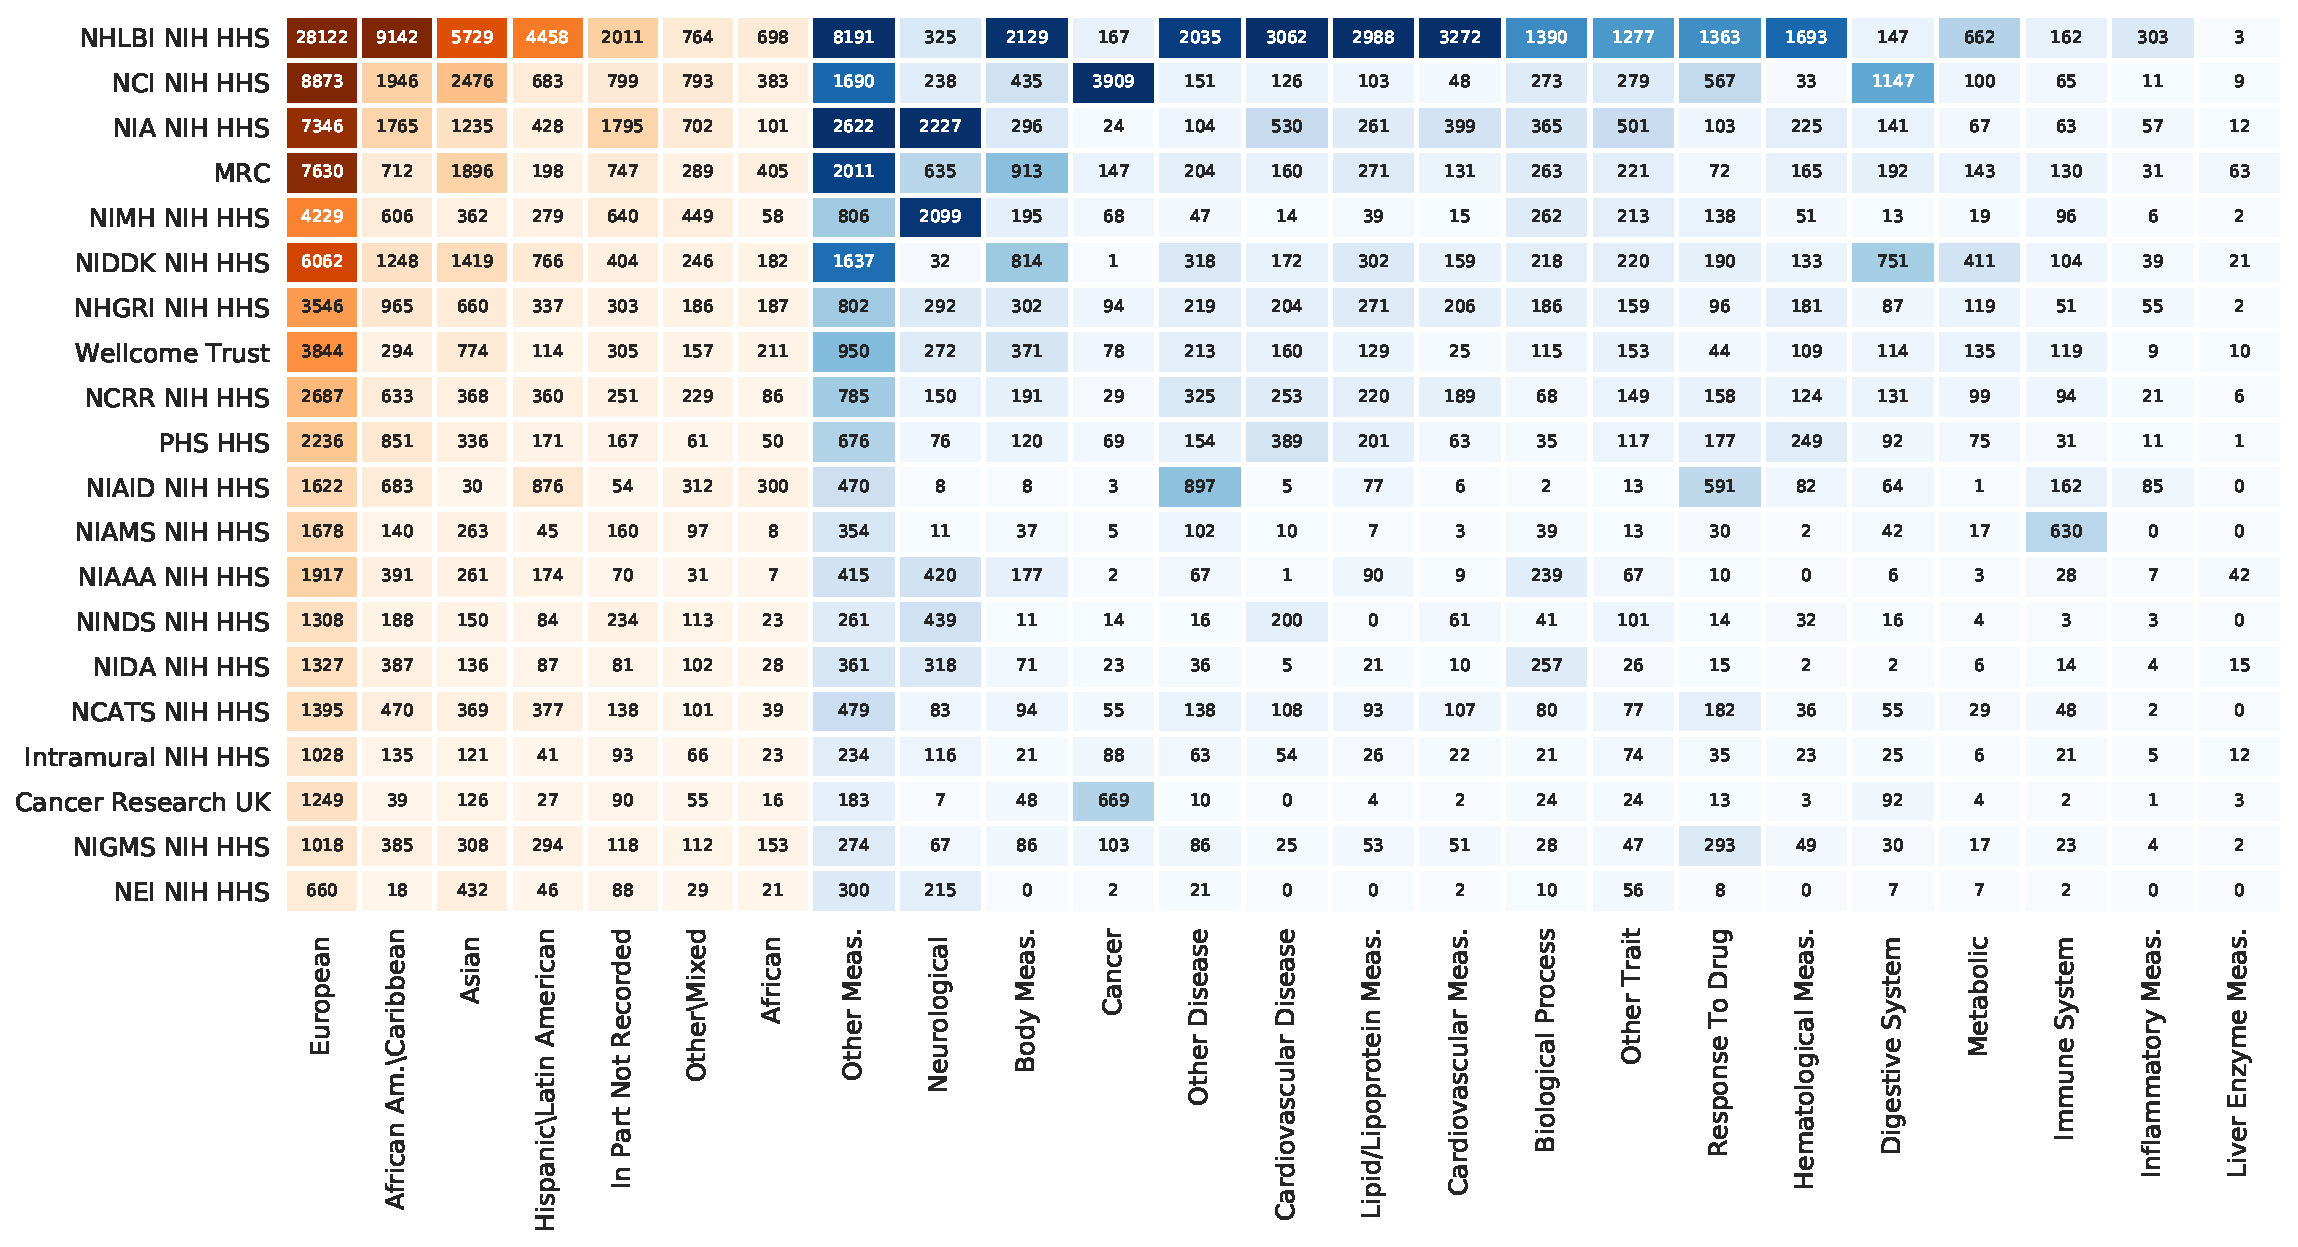
\includegraphics[width=0.925\textwidth, angle=0]{Funder_Heatmap.pdf}
\end{figure}
\end{center}
}

\section{Researchers}
\subsection{}
\frame{
\frametitle{Who are the Most Prolific and Central Authors?}
\vspace{-.2in}\begin{table}[]
\centering
\scalebox{0.7}{
\label{my-label}
\begin{tabular}{rccccccc}\toprule
Author & Papers & Cites & GWAS-H & Between & Degree & Country     & Institution           \\ \midrule
K. Stefansson        & 165    & 24434        & 81     & 0.022       & 0.311  & Iceland     & deCode \\
U. Thorsteinsdottir & 132    & 21063        & 74     & 0.007       & 0.246  & Iceland     & deCode  \\
A. G. Uitterlinden   & 257    & 19893        & 72     & 0.017       & 0.353  & Netherlands & Erasmus MC            \\
A. Hofman          & 255    & 21988        & 72     & 0.014       & 0.342  & U.S.        & Harvard \\
C. M van Duijn   & 175    & 17795        & 67     & 0.008       & 0.284  & Netherlands & UMC Rotterdam         \\
C. Gieger       & 155    & 19353        & 66     & 0.012       & 0.274  & Germany     & Helmholtz-Muenchen    \\
H-E. Wichmann       & 109    & 18395        & 66     & 0.009       & 0.233  & Germany     & Helmholtz-Muenchen    \\
G. Thorleifsson    & 112    & 18084        & 66     & 0.007       & 0.235  & Iceland     & deCode   \\
P. Deloukas         & 96     & 16812        & 62     & 0.007       & 0.229  & U.K.        & Queen Mary UoL        \\
F. Rivadeneira   & 184    & 15537        & 62     & 0.008       & 0.277  & Netherlands & UMC Rotterdam  \\ \bottomrule
\end{tabular}}
\end{table}\vspace{-.1in}
\begin{itemize}\footnotesize
\item GWAS H-Index: published $h$ papers each of which has at least $h$ citations, but only for papers in the Catalog (cites can be from anywhere). \\ \vspace{0.025in}
\item All these authors are either proprietors of large datasets or cohort leaders. \\ \vspace{0.025in}
\item These metrics are highly correlated in general ($\rho>$=0.5).\\ \vspace{0.025in}
\item Slightly further down the list are some close friends of the department, such as: Augustine Kong (28, deCODE and BDI), Cecilia Lindgren (144, BDI) and John Perry (150, Cambridge).
\end{itemize}
}


\subsection{}
\frame{
\frametitle{Structural Gender Bias in Authorship Position}
\begin{itemize}
\item Only 2 of 10 authors above are female, leading us to consider gender bias.\\ \vspace{0.05in}
\item A number of excellent studies discuss gender imbalance in science.\\ \vspace{0.05in}
\item We use a carefully prepared international name dictionary (40,000 entries).\\ \vspace{0.05in}
\item Men contribute 63.05\% of GWAS authorships: 59.53\% of unique authors.\\ \vspace{0.05in}
\item Compare to recent estimates that 72.73\% of academic authorships between 1990-2011 are male.\\ \vspace{0.05in}
\begin {itemize}
\item This increases to 71.70\% filtering for Molecular and Cell Biology.\\ \vspace{0.05in}
\item And to 67.6\% for the specific subdiscipline of Human Genomics.\\ \vspace{0.05in}
\end{itemize}
\item Most importantly we show substantial variation across authorship position: \\ \vspace{0.05in}
\begin{itemize}
\item 56.70\% authors in ‘first author’ (typically junior/post-doc) are female. \\ \vspace{0.05in}
\item Increases to 71.73\% for authorships in the senior ‘last author’ position. \\ \vspace{0.05in}
\end{itemize}
\end{itemize}
}

\subsection{}
\frame{
\frametitle{Gendered Study of Traits}
\begin{center}
\begin{figure}
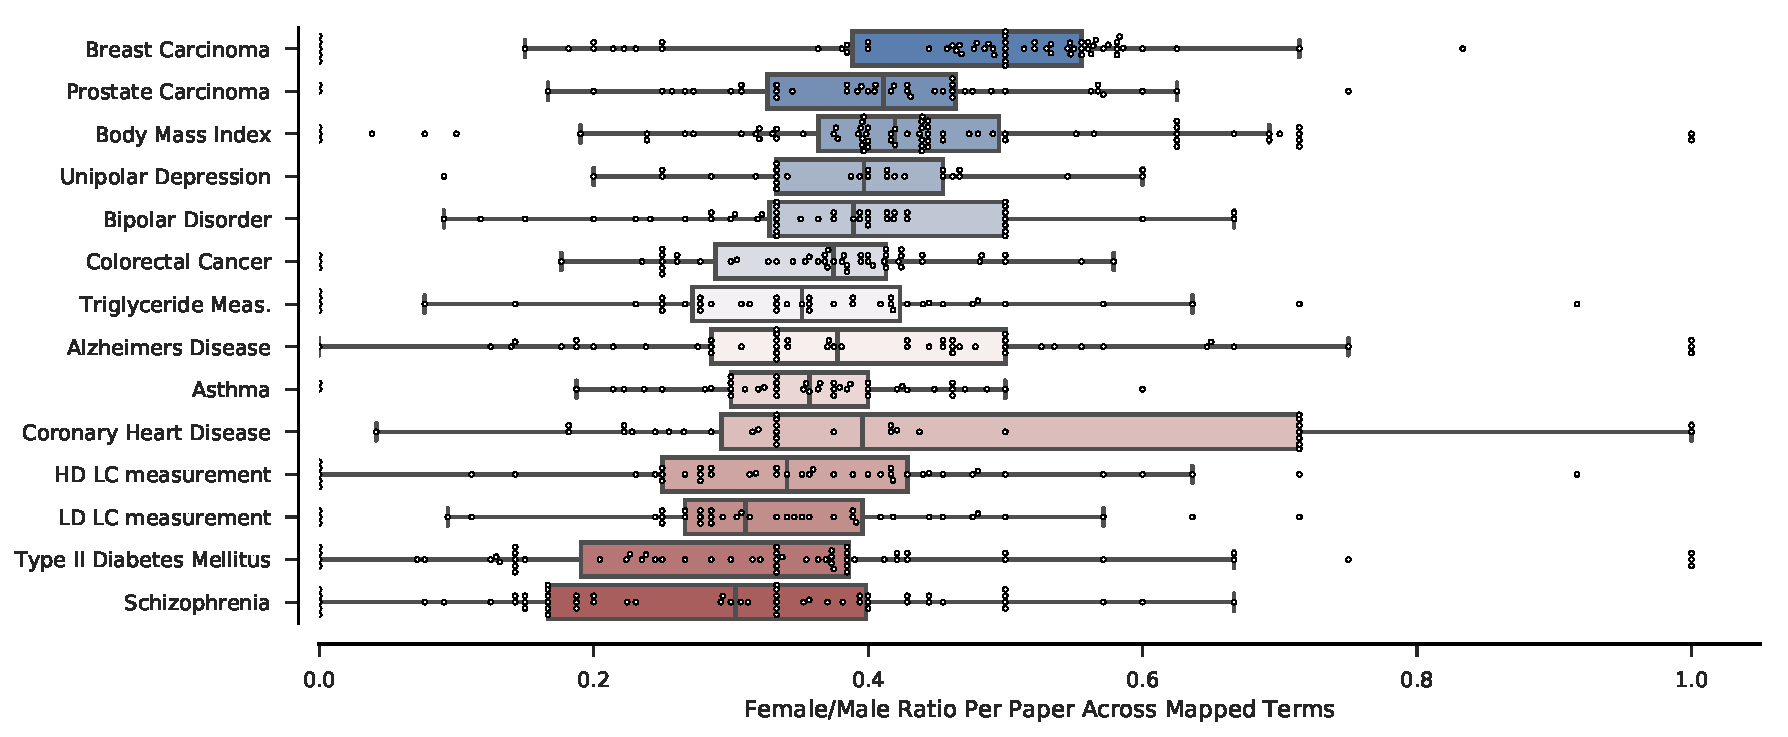
\includegraphics[width=0.925\textwidth, angle=0]{Gender_by_Subjects.pdf}
\end{figure}
\end{center}
\begin{itemize}
\item Concentration of female authorship in studies of Breast Carcinoma (50.5\%). \\ \vspace{0.05in}
\item Male authors are concentrated on Schizophrenia and Type II Diabetes. \\ \vspace{0.1in}
\end{itemize}
}

\subsection{}
\frame{
\frametitle{Contributing Collectives (Consortium)}
Finally, we analyze consortiums associated with various PubMed IDs.\vspace{0.05in}
Dictionary based replacement: eg. ‘AGEN’ and ‘AGEN Consortium’ map to same entity.\vspace{0.05in}
\begin{itemize}
\item We see a total of 612 different collectives.\vspace{0.05in}
\item A total of 753 papers are contributed to by at least one collective.\vspace{0.05in}
\item A total of 1429 collective contributions are made. \\ \vspace{0.1in}
\end{itemize}
The most frequently seen Consortium are:
\begin{enumerate}
\setbeamercolor{enumerate subitem}{fg=red!80!black}
\setbeamertemplate{enumerate items}[default]
\item Wellcome Trust Case Control Consortium (42)
\item CHARGE (38)
\item Wellcome Trust Case Control Consortium 2 (32)
\item DIAGRAM (28)
\item LifeLines Cohort Study (28)
\end{enumerate}
}

\section{Conclusion}
\subsection{}
\frame{
\frametitle{Conclusion}
\begin{itemize}

\item Existing reviews are mostly narrative or extremely narrow commentaries. \\ \vspace{0.1in}
\item Our genetic knowledge base is limited to UK, US and Icelandic particpants. \\ \vspace{0.1in}
\item Structural clusterings of power in authorship and divides of gender. \\ \vspace{0.1in}
\item We develop tools to analyze genomics as it enters the exome sequencing era. \\ \vspace{0.1in}
\item We predict that UK Biobank (94\% `white') and 23andMe (77\% European) will decrease diversity further before it increases. \\ \vspace{0.1in}
\item Two scientometric recomendations:
\begin{enumerate}
\setbeamercolor{enumerate subitem}{fg=red!80!black}
\setbeamertemplate{enumerate items}[default]
\item Mandate ORCID registration and make them a standard return from bibliometric APIs.\\ \vspace{0.025in}
\item Register each cohort with a unique DOI.
\end{enumerate}
\end{itemize}
}






\frame{
\frametitle{}
\frametitle{Looking forward to all and any questions!}

\begin{figure}
\centering
\begin{minipage}{.2\textwidth}
  \centering
\hspace{-.3in}  \includegraphics[width=.75\linewidth]{questionmark.png}
  \label{fig:test1}
\end{minipage}\hspace{-.15in}
\begin{minipage}{.2\textwidth}
  \centering
\hspace{-.3in}  \includegraphics[width=.75\linewidth]{questionmark.png}
  \label{fig:test1}
\end{minipage}\hspace{-.15in}
\begin{minipage}{.2\textwidth}
  \centering
\hspace{-.3in}  \includegraphics[width=.75\linewidth]{questionmark.png}
  \label{fig:test1}
\end{minipage}\hspace{-.15in}
\begin{minipage}{.2\textwidth}
  \centering
\hspace{-.3in}  \includegraphics[width=.75\linewidth]{questionmark.png}
  \label{fig:test1}
\end{minipage}\hspace{-.15in}
\begin{minipage}{.2\textwidth}
  \centering
\hspace{-.3in}  \includegraphics[width=.75\linewidth]{questionmark.png}
  \label{fig:test1}
\end{minipage}\hspace{-.15in}
\end{figure}
\begin{itemize}
\item Thanks again to Pilar, Domant\`{e}, Xuejie and Melinda. \\ \vspace{0.025in}
\item Thanks also to Felix Tropf, Aaron Reeves,  Ben Domingue and the Sociogenome reading group for all their useful comments.\\ \vspace{0.025in}
\item A couple of key references:
\setbeamertemplate{enumerate items}[default]
\begin{enumerate}\tiny
\item A. B. Popejoy et al., Genomics is failing on diversity. Nature. 538, 161–164 (2016)\vspace{0.025in}
\item J. D. West, J. Jacquet, M. M. King, S. J. Correll, C. T. Bergstrom, The Role of Gender in Scholarly Authorship. PLoS One. 8 (2013), doi:10.1371/journal.pone.0066212
\end{enumerate}
\end{itemize}
}


\end{document}